% This file was created by tikzplotlib v0.9.8.
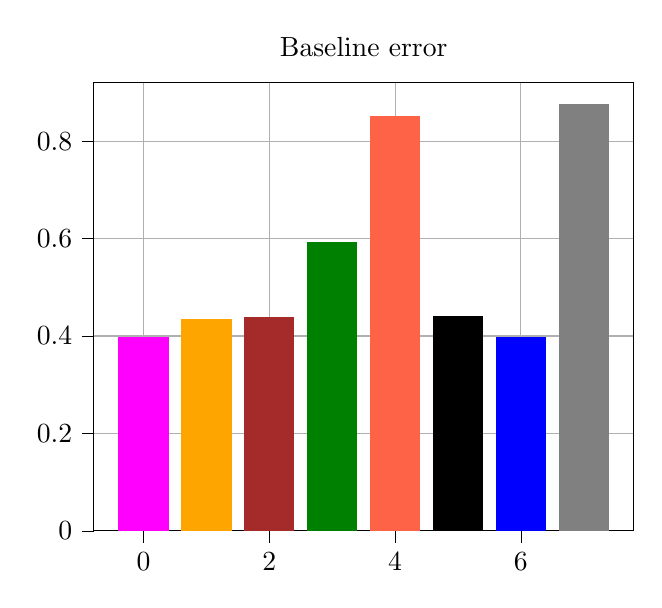
\begin{tikzpicture}

\definecolor{color0}{rgb}{1,0,1}
\definecolor{color1}{rgb}{1,0.647058823529412,0}
\definecolor{color2}{rgb}{0.647058823529412,0.164705882352941,0.164705882352941}
\definecolor{color3}{rgb}{1,0.388235294117647,0.27843137254902}

\begin{axis}[
tick align=outside,
tick pos=left,
title={Baseline error},
x grid style={white!69.0196078431373!black},
xmajorgrids,
xmin=-0.79, xmax=7.79,
xtick style={color=black},
y grid style={white!69.0196078431373!black},
ymajorgrids,
ymin=0, ymax=0.92027027027027,
ytick style={color=black}
]
\draw[draw=none,fill=color0] (axis cs:-0.4,0) rectangle (axis cs:0.4,0.398581081081081);
\draw[draw=none,fill=color1] (axis cs:0.6,0) rectangle (axis cs:1.4,0.435472972972973);
\draw[draw=none,fill=color2] (axis cs:1.6,0) rectangle (axis cs:2.4,0.438513513513514);
\draw[draw=none,fill=green!50.1960784313725!black] (axis cs:2.6,0) rectangle (axis cs:3.4,0.593310810810811);
\draw[draw=none,fill=color3] (axis cs:3.6,0) rectangle (axis cs:4.4,0.850878378378378);
\draw[draw=none,fill=black] (axis cs:4.6,0) rectangle (axis cs:5.4,0.441216216216216);
\draw[draw=none,fill=blue] (axis cs:5.6,0) rectangle (axis cs:6.4,0.397432432432432);
\draw[draw=none,fill=white!50.1960784313725!black] (axis cs:6.6,0) rectangle (axis cs:7.4,0.876447876447876);
\end{axis}

\end{tikzpicture}
